\documentclass[journal]{IEEEtran}
\usepackage[a5paper, margin=10mm, onecolumn]{geometry}
\usepackage{amsmath,amssymb,amsfonts,amsthm}
\usepackage{gvv-book}
\usepackage{gvv}
\usepackage{hyperref}

\begin{document}

\title{10.7.75}
\author{Puni Aditya - EE25BTECH11046}
\maketitle

\textbf{Question:}
Find the equations of tangents drawn from origin to the circle $x^2+y^2-2rx-2hy+h^2=0$,are
\begin{multicols}{2}
\begin{enumerate}
    \item $x=0$
    \item $y=0$
    \item $\brak{h^2-r^2}x-2rhy=0$
    \item $\brak{h^2-r^2}x+2rhy=0$
\end{enumerate}
\end{multicols}

\textbf{Solution:}

A general conic section is described by the equation
\begin{align}
    \vec{x}^\top \vec{V} \vec{x} + 2\vec{u}^\top \vec{x} + f = 0
\end{align}
where $\vec{V}$ is a symmetric matrix. A line passing through a point $\vec{h}$ and having unit direction vector $\vec{m}$ is
\begin{align}
    \vec{x} = \vec{h} + k\vec{m}
\end{align}
Substitute the line equation into the conic to find points of intersection.
\begin{align}
    k^2\brak{\vec{m}^\top\vec{V}\vec{m}} + 2k\brak{\vec{m}^\top\vec{V}\vec{h} + \vec{u}^\top\vec{m}} + \brak{\vec{h}^\top\vec{V}\vec{h} + 2\vec{u}^\top\vec{h} + f} = 0
\end{align}
For the line to be tangent to the conic, the discriminant of quadratic in $k$ must be zero. \\
Let $g\brak{\vec{h}} = \vec{h}^\top\vec{V}\vec{h} + 2\vec{u}^\top\vec{h} + f$ be the value of the conic expression at the point $\vec{h}$.
\begin{align}
    \brak{\vec{m}^\top\vec{V}\vec{h} + \vec{u}^\top\vec{m}}^2 - \brak{\vec{m}^\top\vec{V}\vec{m}}\brak{g\brak{\vec{h}}} = 0
\end{align}
\begin{align}
    \brak{\vec{m}^\top \brak{\vec{V}\vec{h} + \vec{u}}}^2 - g\brak{\vec{h}}\brak{\vec{m}^\top\vec{V}\vec{m}} &= 0 \\
    \vec{m}^\top \brak{\brak{\vec{V}\vec{h} + \vec{u}}\brak{\vec{V}\vec{h} + \vec{u}}^\top} \vec{m} - \vec{m}^\top \brak{g\brak{\vec{h}}\vec{V}} \vec{m} &= 0 \\
    \vec{m}^\top \sbrak{\brak{\vec{V}\vec{h} + \vec{u}}\brak{\vec{V}\vec{h} + \vec{u}}^\top - \brak{\vec{h}^\top\vec{V}\vec{h} + 2\vec{u}^\top\vec{h} + f}\vec{V}} \vec{m} &= 0
\end{align}
\begin{align}
    \text{Let }\vec{\Sigma} = \brak{\vec{V}\vec{h} + \vec{u}}\brak{\vec{V}\vec{h} + \vec{u}}^\top - \brak{\vec{h}^\top\vec{V}\vec{h} + 2\vec{u}^\top\vec{h} + f}\vec{V} \label{eq:sigma_notation}
\end{align}
\begin{align}
    \vec{m}^\top \vec{\Sigma} \vec{m} = 0 \label{eq:sigma}
\end{align}
This is the general equation for the directions of tangents from an arbitrary point $\vec{h}$.

For $\vec{h} = \vec{0}$,
\begin{align}
    \vec{\Sigma} = \brak{\vec{V}\vec{0} + \vec{u}}\brak{\vec{V}\vec{0} + \vec{u}}^\top - \brak{\vec{0}^\top\vec{V}\vec{0} + 2\vec{u}^\top\vec{0} + f}\vec{V} = \vec{u}\vec{u}^\top - f\vec{V}
\end{align}

To solve this, the symmetric matrix $\vec{\Sigma}$ is diagonalized. The eigendecomposition of $\vec{\Sigma}$ is $\vec{\Sigma} = \vec{P}\vec{D}\vec{P}^\top$, where: \\
$\vec{D}$ is a diagonal matrix with the eigenvalues of $\vec{\Sigma}$ on its diagonal
\begin{align}
    \vec{D} = \myvec{\lambda_1 & 0 \\ 0 & \lambda_2} \label{eq:1}
\end{align}
$\vec{P}$ is an orthogonal matrix whose columns are the corresponding orthonormal eigenvectors. So, $\vec{P}^\top \vec{P} = \vec{P}\vec{P}^\top = 1$.
\begin{align}
    \vec{P} = \myvec{\vec{v_1} & \vec{v_2}} \label{eq:2}
\end{align}
Substitute \eqref{eq:1} and \eqref{eq:2} in \eqref{eq:sigma}
\begin{align}
    \vec{m}^\top (\vec{P}\vec{D}\vec{P}^\top) \vec{m} = 0
\end{align}
\begin{align}
	\vec{m} = \vec{P}\myvec{\sqrt{\abs{\lambda_2}} \\ \pm\sqrt{\abs{\lambda_1}}} \label{eq:eigenmat}
\end{align}

For the circle $x^2+y^2-2rx-2hy+h^2=0$,
\begin{align}
    \vec{A} = \myvec{1 & 0 \\ 0 & 1},\text{ }\vec{u} = \myvec{-r \\ -h},\text{ }f = h^2
\end{align}
From \eqref{eq:sigma_notation},
\begin{align}
    \vec{\Sigma} = \myvec{-r \\ -h}\myvec{-r & -h} - h^2\myvec{1 & 0 \\ 0 & 1} = \myvec{r^2-h^2 & rh \\ rh & 0}
\end{align}
The characteristic equation is $\mydet{\vec{\Sigma}-\lambda\vec{I}}=0$. \\
Let $\lambda^2 + a_1 \lambda + a_2 = 0$. Using Faddeev-Leverrier Method,
\begin{align}
    \vec{B_1} &= \vec{A} \\
    a_1 &= - tr\brak{\vec{B_1}} = -\brak{r^2-h^2}
\end{align}
\begin{align}
    \vec{B_2} &= \vec{A}\brak{\vec{B_1} + a_1\vec{I}} \\
    \vec{B_2} &= \myvec{r^2h^2 & 2rh\brak{r^2-h^2} \\ 0 & r^2h^2} \\
    a_2 &= -\frac{1}{2}tr\brak{\vec{B_2}} \\
    a_2 &= -r^2h^2
\end{align}
So, $\lambda^2 - \brak{r^2-h^2}\lambda - r^2h^2 = 0$, giving the eigenvalues $\lambda_1 = r^2$ and $\lambda_2 = -h^2$.
\begin{align}
    \vec{P} = \frac{1}{\sqrt{r^2+h^2}}\myvec{r & h \\ h & -r}
\end{align}
Using \eqref{eq:eigenmat},
\begin{align}
    \vec{m_1} &= \frac{1}{\sqrt{r^2+h^2}}\myvec{r & h \\ h & -r}\myvec{\sqrt{\abs{-h^2}} \\ \sqrt{\abs{r^2}}} \\
    &= \frac{1}{\sqrt{r^2+h^2}}\myvec{r & h \\ h & -r}\myvec{h \\ r} \\
    &= \frac{1}{\sqrt{r^2+h^2}}\myvec{2rh \\ h^2-r^2} \label{eq:equation1}
\end{align}
\begin{align}
    \vec{m_1} &= \frac{1}{\sqrt{r^2+h^2}}\myvec{r & h \\ h & -r}\myvec{\sqrt{\abs{-h^2}} \\ -\sqrt{\abs{r^2}}} \\
    &= \frac{1}{\sqrt{r^2+h^2}}\myvec{r & h \\ h & -r}\myvec{h \\ -r} \\
    &= \frac{1}{\sqrt{r^2+h^2}}\myvec{0 \\ h^2+r^2} \label{eq:equation2}
\end{align}
For $\vec{m_1}$, $\brak{h^2-r^2}x - \brak{2rh}y = 0$. This is option \textbf{3}. \\
For $\vec{m_2}$, $\brak{r^2+h^2} \times x - 0 \times y = 0 \implies x = 0$. This is option \textbf{1}. \\
So, options \textbf{\brak{1}} and \textbf{\brak{3}} are true.

\textbf{Example:}\\
Let r = 3, h = 2. \\
For the circle $x^2+y^2-6x-4y+4=0$,
\begin{align}
    \vec{A} = \myvec{1 & 0 \\ 0 & 1},\text{ }\vec{u} = \myvec{-3 \\ -2},\text{ }f = 4
\end{align}
From \eqref{eq:sigma_notation},
\begin{align}
    \vec{\Sigma} = \myvec{-3 \\ -2}\myvec{-3 & -2} - 4\myvec{1 & 0 \\ 0 & 1} = \myvec{5 & 6 \\ 6 & 0}
\end{align}
The characteristic equation is $\mydet{\vec{\Sigma}-\lambda\vec{I}}=0$. \\
Let $\lambda^2 + a_1 \lambda + a_2 = 0$. Using Faddeev-Leverrier Method,
\begin{align}
    \vec{B_1} &= \vec{A} \\
    a_1 &= - tr\brak{\vec{B_1}} = -\brak{5}
\end{align}
\begin{align}
    \vec{B_2} &= \vec{A}\brak{\vec{B_1} + a_1\vec{I}} \\
    \vec{B_2} &= \myvec{36 & 60 \\ 0 & 36} \\
    a_2 &= -\frac{1}{2}tr\brak{\vec{B_2}} \\
    a_2 &= -36
\end{align}
So, $\lambda^2 - 5\lambda - 36 = 0$, giving the eigenvalues $\lambda_1 = 9$ and $\lambda_2 = -4$.
\begin{align}
    \vec{P} = \frac{1}{\sqrt{13}}\myvec{3 & 2 \\ 2 & -3}
\end{align}
Using \eqref{eq:equation1} and \eqref{eq:equation2},
\begin{align}
    \vec{m_1} &= \frac{1}{\sqrt{13}}\myvec{12 \\ -5} \\
    \vec{m_2} &= \frac{1}{\sqrt{13}}\myvec{0 \\ 13}
\end{align}
For $\vec{m_1}$, $\brak{-5}x - \brak{12}y = 0$. This is option \textbf{3}. \\
For $\vec{m_2}$, $13 \times x - 0 \times y = 0 \implies x = 0$. This is option \textbf{1}. \\
So, options \textbf{\brak{1}} and \textbf{\brak{3}} are true.

\begin{figure}[h!]
	\centering
	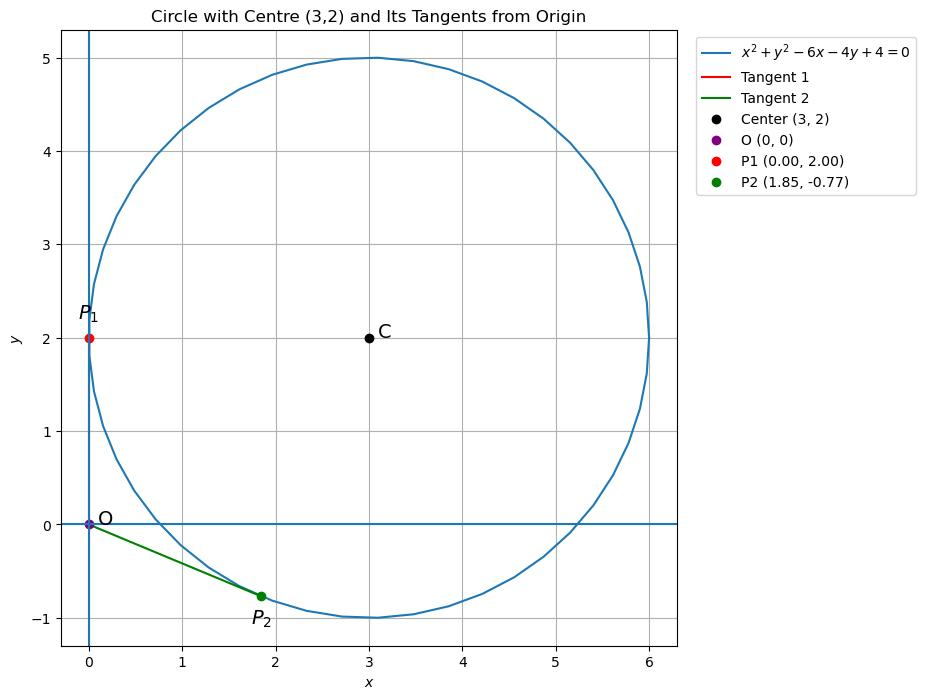
\includegraphics[width=0.9\columnwidth]{figs/plot_c.jpg}
	\caption*{Example}
	\label{fig:example}
\end{figure}

\end{document}
